\clearpage
\appendices
\section{Approximation Under Per-Output Error Budgets}
\label{app:sensitivity}
Exact planning never changes an answer. This appendix describes the one opt-in mechanism that does: replacing small rotation angles by zero when a conditional bound guarantees that every requested output stays within its error budget. Its interest for this paper is structural. An accepted substitution can remove a weak bridge between two blocks of a circuit and therefore shrink cones that exact planning has to keep whole.

\subsection{Observable-Error Bound}
\label{sec:sensitivity-theory}
The dense backend retains complex128 amplitudes regardless of angle precision. Parameter approximation can save work when it enables gate cancellation or reduces an observable's causal cone. Our separate sensitivity API explicitly executes shifted circuits, then selects zero-angle substitutions under per-output absolute error budgets. Ordinary planning remains exact and lazy. The following result formalizes its acceptance rule using standard parameter-shift and Taylor arguments~\cite{schuld2019gradients,lerch2026patches}; the experiments motivate and test its application but are not its proof.

\begin{theorem}[Observable error under simultaneous angle changes]
\label{thm:observable-error}
Let $U(\theta)$ be a unitary circuit on a fixed normalized input state, with independently indexed rotation occurrences $R_{P_g}(\theta_g)=\exp(-i\theta_gP_g/2)$, where each $P_g$ is a Pauli operator. For a terminal Pauli $O_k$, define $f_k(\theta)=\operatorname{Tr}[O_kU(\theta)\rho U(\theta)^\dagger]$. Let $C_k$ be its structural backward cone in the unchanged gate topology. For any real occurrence perturbation $\delta$, set $L_k=\sum_{g\in C_k}|\delta_g|$ and $J_{kg}=\partial_g f_k(\theta)$. Then
\begin{equation}
 |f_k(\theta+\delta)-f_k(\theta)|
 \leq\min\{2,L_k,|J_k\delta|+L_k^2/2\}.
 \label{eq:ideal-sensitivity-bound}
\end{equation}
The coefficient $1/2$ in the quadratic remainder is asymptotically sharp over this circuit class. If $|\widehat J_{kg}-J_{kg}|\leq\eta$ inside $C_k$, $\widehat J_{kg}=0$ outside $C_k$, and each numerical endpoint has absolute error at most $\eta$, their difference is bounded by
\begin{equation}
 B_k=\min\{2,L_k,|\widehat J_k\delta|+\eta L_k+L_k^2/2\}+2\eta.
 \label{eq:sensitivity-bound}
\end{equation}
\end{theorem}

The proof and sharpness example are in the Appendix. Occurrences sharing a symbolic parameter count separately. Their derivatives sum by the chain rule; the appropriate shift calculation changes only one occurrence at a time:
\begin{equation}
 J_{kg}=\tfrac12[f_k(\theta+\tfrac\pi2 e_g)-f_k(\theta-\tfrac\pi2 e_g)].
\end{equation}
Two expectation estimates with error at most $\eta$ give derivative error at most $\eta$. The implemented allowance is assumed rather than established by interval arithmetic, and bound computations are not rounded outward. Equation~\eqref{eq:sensitivity-bound} is therefore a conditional mathematical guarantee, not a floating-point certificate. An exactly unchanged relevant circuit has zero approximation change; comparing two separately computed endpoints can still incur numerical error.

\begin{corollary}[Sufficient perturbation radius]
\label{cor:radius}
For a chosen occurrence direction $v$ and $\delta=t v$, let
$\ell_k=\sum_{g\in C_k}|v_g|$,
$a_k=|\widehat J_kv|+\eta\ell_k$, and
$e_k=\epsilon_k-2\eta>0$.
If $\ell_k>0$, a sufficient condition for output error at most $\epsilon_k$ is
\begin{equation}
 |t|\leq\frac{2e_k}{a_k+\sqrt{a_k^2+2\ell_k^2e_k}}.
 \label{eq:safe-radius}
\end{equation}
Taking the minimum radius over the requested outputs satisfies every budget. Outputs with $\ell_k=0$ impose no approximation restriction.
\end{corollary}

This follows by solving $a_k|t|+\ell_k^2t^2/2\leq e_k$. It is a sufficient radius, not the largest admissible one, since the other terms of Eq.~\eqref{eq:sensitivity-bound} can be tighter. In exact arithmetic, if $m_k$ affected occurrences each change by at most $d$, the uniform rule $m_kd\leq\epsilon_k$ always suffices. At a point where all those derivatives vanish, the stronger sufficient rule is $m_kd\leq\sqrt{2\epsilon_k}$. Thus zero gradient permits a larger tolerance but does not justify unlimited pruning. For a nearest rounding grid of spacing $h$, substitute $d=h/2$. These bounds have no explicit $2^n$ factor, but the number of relevant occurrences can grow with the circuit.

\begin{corollary}[Resource reduction after admissible bridge removal]
\label{cor:resource-reduction}
Suppose an admissible perturbation followed by exact rewrites separates a product-zero-input circuit into components of widths $b_j\leq b$, and every requested observable is supported within one component. Simulating each needed component once suffices. If it has $G_j$ fixed-arity gates and $K_j$ requested Pauli outputs, a dense evaluation requires
\begin{equation}
 O\!\left(\sum_j (G_j+1+K_jb_j)2^{b_j}\right)
 \label{eq:reduced-work}
\end{equation}
arithmetic operations. Its largest state payload is at most $16\,2^b$ bytes, or a reduction of at least $2^{W-b}$ relative to a dense plan whose largest state has width $W\geq b$.
\end{corollary}

Factorization of the input and all remaining gates proves the corollary. It concerns the evaluation phase; profiling, search, resident memory and competing tensor-network methods are outside this operation/payload statement. With polynomial gate/output counts and $b=O(\log n)$, the reduced evaluation is polynomial, but this does not establish polynomial cost for obtaining its sensitivity profile. The measured $\mathrm{CX}\,R_Z(\theta)\,\mathrm{CX}$ bridges satisfy the structural hypothesis when all intercomponent bridges are set to zero and cancelled. Small angles without this separation need not reduce width.

\subsubsection{Planning and setup repayment}
The prototype tests at most 64 zeroed subsets, applies Eq.~\eqref{eq:sensitivity-bound} to every output, and retains the exact plan on execution-cost ties. Existing execution scores rank admissible variants; there is no global optimality claim. Profiling and search are recorded separately. For a specified execution policy, let $H_e,H_a$ be exact and approximate setup costs, including profiling in $H_a$, and let $T_e,T_a$ be constant per-collection costs. Approximation improves lifetime precisely when
\begin{equation}
 R(T_e-T_a)>H_a-H_e.
 \label{eq:reuse-condition}
\end{equation}
For positive saving $s=T_e-T_a$ and nonnegative added setup $\Delta H$, the first improving integer horizon is $\lfloor\Delta H/s\rfloor+1$. With variable timings, replace $Rs$ by the cumulative measured savings. This accounting identity is a decision rule, not a hardware speedup theorem. The current implementation reports the required terms; automatic joint selection of profiling effort, reuse horizon and worker count remains open.


\subsection{Detailed Observable-Sensitivity Study}
This benchmark evaluates the implemented acceptance rule of Theorem~\ref{thm:observable-error} and the separation mechanism of Corollary~\ref{cor:resource-reduction}. It retains all profiling and setup charges in the lifetime comparison. The derived radius in Corollary~\ref{cor:radius} is a theoretical planning rule; the measured candidate search instead tests explicit zero-angle subsets.

\subsubsection{Validation design}
An independent NumPy oracle checks 96 seeded, noncommuting circuits of two to five qubits. Six simultaneous rotation perturbations at scales $10^{-6}$, $10^{-3}$, $0.1$, and $1$ radian give 384 perturbation vectors and 1,152 observable comparisons. Derivatives are independently checked with central differences at step $10^{-5}$. Separate analytic controls cover shared parameters, stationary points, and cancellation as the finite-difference step approaches machine precision.

The performance study uses nine fixtures: two local blocks at total widths 8 and 12; three seeds of two-block width 16 and three-block width 15; and a connected 16-qubit control. Each has 20 random local preparation layers, weak $\mathrm{CX}\,R_Z(\delta)\,\mathrm{CX}$ bridges with $\delta=0.003$ or $0.006$, and four further noncommuting local layers. The control retains an extra CX bridge after approximation. Requests are local $X$ and $Z$ outputs, two per block. The candidate ablation compares exact execution, uniform rounding of the eligible bridge angles to a $0.02$-radian grid, gradient-only acceptance, and bounded selection at budgets $10^{-6}$, $10^{-4}$, and $10^{-2}$.

Three sequential interpreter sessions use a frozen source snapshot, 1/2/4 local workers, and one native thread per process. Each policy has one first collection and seven interleaved warm collections; all original and modified outputs are checked independently. Lifetime comparisons charge profiling, search, startup and shutdown over eight collections at budget $0.01$. Common program construction and validation-oracle work are excluded. The same measured pool setup is charged to both counterfactual workflows. Separate resource probes report payload and sampled parent-plus-pool RSS. Repeated sessions do not add independent circuit seeds.

\subsubsection{Accuracy and execution results}
No conditional-bound violation occurs in the 1,152 independent observable comparisons. The linear predictor underestimates the observed change by more than $10^{-12}$ in 373 comparisons; these are prediction underestimates, not acceptance-budget violations. Maximum disagreement between occurrence shifts and the independent finite differences is $3.75\times10^{-11}$. In the analytic single-qubit step sweep at $\theta=0.37$, central differences have derivative error $6.03\times10^{-10}$ at step $10^{-4}$, but $0.362$ at step $10^{-16}$, where subtraction returns zero. Parameter shift has error $5.55\times10^{-17}$ on this fixture. This illustrates cancellation, not a universal optimal finite-difference step.

Uniform rounding violates the $10^{-6}$ budget on all nine timing fixtures and the $10^{-4}$ budget on four. Bounded selection has no observed violations and changes zero and five fixtures, respectively; at $0.01$, it changes all nine. Gradient-only acceptance has no budget violation in this small weak-bridge sweep, but fails the separate stationary-point counterexample. These controls support including a remainder term without claiming that every small-gradient approximation fails. Across 1,134 warm collections, 162 first collections and 162 resource probes, the maximum native disagreement with the corresponding original or modified NumPy reference is $1.24\times10^{-15}$; approximation bias is reported separately.

On the two-block 16-qubit fixtures, approximation reduces the largest state from 16 to eight qubits ($256\times$ payload reduction). Serial warm execution falls from 63.21--67.36\,ms to 1.17--1.65\,ms across sessions and seeds, giving $40.56\times$--$53.88\times$. However, profiling costs 133.05--165.46\,ms. The eight-collection lifetime speedup is consequently $2.89\times$--$3.57\times$, with observed sustained break-even in two to three collections. Maximum approximation bias is $1.14\times10^{-5}$, below a maximum conditional bound of $1.62\times10^{-5}$. Two workers lower profiling to 87.83--103.89\,ms, but the small approximate tasks and process setup limit lifetime speedup to $2.27\times$--$2.57\times$.

Three-block 15-qubit fixtures reduce maximum width to five ($1024\times$ payload reduction), with maximum observed bias $2.06\times10^{-4}$. Serial warm speedups of $30.95\times$--$35.46\times$ become $1.31\times$--$1.55\times$ after all charges. Four-worker lifetime results span $0.99\times$--$1.10\times$. The eight-qubit cases regress over eight collections at every worker count. The connected 16-qubit control retains width 16 and has lifetime ratios of $0.77\times$--$0.85\times$ despite admissible angle changes. Thus angle approximation needs both exploitable structure and enough reuse to repay analysis.

Figure~\ref{fig:sensitivity} presents error control and charged execution; Table~\ref{tab:sensitivity-results} retains all fixture/worker families in the Appendix. Payload reductions do not imply comparable RSS reductions: in the serial 16-qubit weak-bridge probes, both policies retain approximately 51--52\,MiB sampled RSS. Four workers raise the sampled parent-plus-pool sum to approximately 220--223\,MiB. Allocator retention and shared-page accounting limit interpretation. RQ4 has positive evidence on constructed weak bridges, with explicit negative controls; it does not establish general variational-circuit acceleration or automatic selection of approximation and worker policies.

\begin{figure*}[t]
\centering
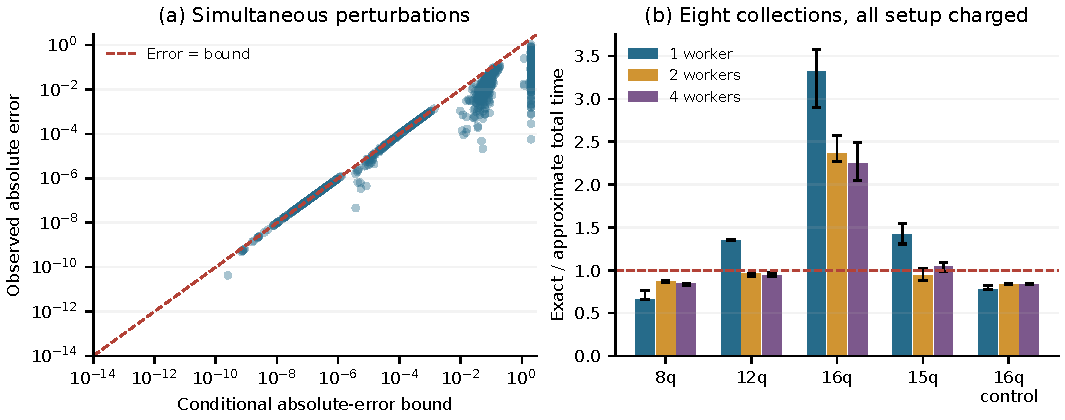
\includegraphics[width=0.98\textwidth]{figures/sensitivity_tradeoff.pdf}
\caption{Observable-sensitivity validation. (a) Actual errors versus conditional bounds for simultaneous perturbations; zero points are omitted on logarithmic axes. (b) Median eight-collection lifetime ratios, with whiskers spanning session/seed configurations rather than confidence intervals. Each ratio compares exact and approximate execution at the same worker count. Profiling, search and worker setup/shutdown are charged.}
\label{fig:sensitivity}
\end{figure*}



% Generated by benchmarks/plot_sensitivity.py from validated summary.json.
\begin{table*}[t]
\centering
\caption{Sensitivity study: ranges across three interpreter sessions and the stated seeds. Warm speedups compare exact and bounded execution at equal worker counts. Lifetime charges eight collections, profiling, search and pool setup/shutdown. Payload is the largest individual complex128 state, not RSS. Budget: $0.01$ per output.}
\label{tab:sensitivity-results}
\footnotesize
\begin{tabular}{lrrrrrrr}
\toprule
Fixture & Seeds & Workers & Width & Payload factor & Warm speedup & Lifetime speedup & Profile (ms) \\
\midrule
8q / 2 blocks & 1 & 1 & $8\to 4$ & 16 & 2.23--2.40 & 0.66--0.76 & 7.50--8.07 \\
8q / 2 blocks & 1 & 2 & $8\to 4$ & 16 & 1.58--2.64 & 0.86--0.88 & 21.80--36.20 \\
8q / 2 blocks & 1 & 4 & $8\to 4$ & 16 & 1.16--1.79 & 0.82--0.85 & 25.95--28.15 \\
12q / 2 blocks & 1 & 1 & $12\to 6$ & 64 & 4.80--5.18 & 1.35--1.35 & 11.17--13.00 \\
12q / 2 blocks & 1 & 2 & $12\to 6$ & 64 & 2.48--3.66 & 0.93--0.97 & 21.71--24.60 \\
12q / 2 blocks & 1 & 4 & $12\to 6$ & 64 & 2.46--2.84 & 0.93--0.98 & 21.76--24.11 \\
16q / 2 blocks & 3 & 1 & $16\to 8$ & 256 & 40.56--53.88 & 2.89--3.57 & 133.05--165.46 \\
16q / 2 blocks & 3 & 2 & $16\to 8$ & 256 & 27.43--31.70 & 2.27--2.57 & 87.83--103.89 \\
16q / 2 blocks & 3 & 4 & $16\to 8$ & 256 & 22.70--30.28 & 2.04--2.49 & 89.91--109.28 \\
15q / 3 blocks & 3 & 1 & $15\to 5$ & 1024 & 30.95--35.46 & 1.31--1.55 & 138.32--158.77 \\
15q / 3 blocks & 3 & 2 & $15\to 5$ & 1024 & 9.31--12.51 & 0.88--1.02 & 138.80--181.29 \\
15q / 3 blocks & 3 & 4 & $15\to 5$ & 1024 & 11.86--17.78 & 0.99--1.10 & 106.85--137.25 \\
16q connected control & 1 & 1 & $16\to 16$ & 1 & 0.92--1.03 & 0.77--0.82 & 138.56--165.83 \\
16q connected control & 1 & 2 & $16\to 16$ & 1 & 0.97--1.00 & 0.83--0.85 & 106.49--130.78 \\
16q connected control & 1 & 4 & $16\to 16$ & 1 & 0.99--1.01 & 0.83--0.84 & 108.31--126.78 \\
\bottomrule
\end{tabular}
\end{table*}


\subsection{Proof of Theorem~\ref{thm:observable-error}}
\begin{IEEEproof}
For a Pauli rotation channel $\mathcal U_g$, define $\mathcal D_g(A)=-i[P_g/2,A]$. Then $\partial_g\mathcal U_g=\mathcal D_g\mathcal U_g$ and $\partial_g^2\mathcal U_g=\mathcal D_g^2\mathcal U_g$. Since $\|P_g\|_\infty=1$,
\begin{equation}
 \|\mathcal D_g(A)\|_1\leq\|P_gA\|_1/2+\|AP_g\|_1/2\leq\|A\|_1.
\end{equation}
Every unitary channel preserves trace norm. Differentiating a circuit once or twice inserts one or two such derivative maps. This also covers two derivatives of the same occurrence. Using $\|\rho\|_1=1$ and $|\operatorname{Tr}(O_k A)|\leq\|O_k\|_\infty\|A\|_1$ therefore gives
\begin{equation}
 |\partial_g f_k(\vartheta)|\leq1,\qquad
 |\partial_g\partial_h f_k(\vartheta)|\leq1
 \label{eq:uniform-derivative-bounds}
\end{equation}
at every angle vector $\vartheta$, not only the profiled point. A structural backward cone contains every gate that can affect the evolved observable. Changing angles leaves gate supports fixed, so derivatives involving an occurrence outside $C_k$ vanish identically.

Put $q(t)=f_k(\theta+t\delta)$. Equation~\eqref{eq:uniform-derivative-bounds} implies $|q'(t)|\leq L_k$ and $|q''(t)|\leq L_k^2$. Taylor's integral identity gives
\begin{equation}
 q(1)-q(0)=J_k\delta+\int_0^1(1-t)q''(t)\,dt.
\end{equation}
Taking absolute values bounds the remainder by $L_k^2/2$. Integrating the first-derivative bound yields $L_k$, while the range of a norm-one observable yields two. Taking their minimum proves Eq.~\eqref{eq:ideal-sensitivity-bound}.

For sharpness, compose $m$ single-qubit $R_Y$ occurrences on $|0\rangle$, all at zero, and request $Z$. Perturb every occurrence by $d$. The gradient at the starting point vanishes, but the output change is $1-\cos(md)$ with $L=m|d|$. Consequently,
\begin{equation}
 \lim_{d\to0}\frac{1-\cos(md)}{(m d)^2}=\frac12.
\end{equation}
No smaller uniform coefficient can replace $1/2$ in the quadratic remainder. The same example shows why counting shared occurrences is necessary. Expanding around a total rotation of $\pi/2$ similarly saturates the linear bound to first order.

Finally, with the structural zeros enforced, $|(\widehat J_k-J_k)\delta|\leq\eta L_k$. Adding this to the Taylor term and allowing error $\eta$ at each independently evaluated endpoint proves Eq.~\eqref{eq:sensitivity-bound}. This last step is conditional on the stated numerical error bounds and exact evaluation of the bound expression itself.
\end{IEEEproof}

The theorem is an application of unitary derivative bounds and Taylor's integral remainder, not an inference from a finite sample. The two corollaries add sufficient precision and reduced-evaluation conditions for this planner. The experiments validate particular implementations and timing hypotheses; they do not establish a universal speedup or the novelty of the underlying mathematical inequalities.

\subsection{Sensitivity Reproducibility}

The implementation assumes $\eta=10^{-10}$ in the study. Independent double-precision agreement does not prove this allowance or establish outward rounding of the computed bound. The bound is consequently an analytic error-control rule with an explicit numerical assumption. The evaluated program must already be feasible; neither small gradients nor approximate candidates supply otherwise unavailable exact profiles.

\path{src/lazyqc/sensitivity.py} implements profiling and bounded candidate search. \path{benchmarks/run_sensitivity.py} defines the cases; \path{tests/test_sensitivity.py} includes independent dense-matrix and analytic regression tests. Raw final observations reside in \path{results/sensitivity/session0/} through \path{results/sensitivity/session2/}; \path{results/sensitivity/frozen_source/} contains their measured source snapshot. Pilot runs are excluded from aggregation. \path{benchmarks/summarize_sensitivity.py} validates source hashes and produces the summary; \path{docs/SENSITIVITY.md} specifies cost scopes and reproduction. Native thread counts are fixed at one on the same unpinned, heterogeneous i7-13700H host used for the local-worker study. Summed RSS includes shared pages more than once and may retain allocations from earlier exact collections.


\section{Earlier Planning Studies}
\label{app:earlier}
The studies in this appendix predate the QML evaluation. They use small QAOA-derived fixtures and compare planning policies with each other rather than with direct execution, which is why they are not part of the main results. They remain useful because they isolate the cost of search, the value of joint cut selection and the role of expected reuse.

\subsection{Two-policy selection with expected reuse}
Before the QML study, we evaluated whether historical timing can decide between independent request optimization followed by deduplication (B3) and joint group, rewrite and cut search (B5) for a declared number of collections $R\in\{1,2,4,\dots,512\}$. For each policy $p$, a reconstructed lifetime $\widetilde L_p(R)=\operatorname{median}(H_p)+R\operatorname{median}(T^{\mathrm{warm}}_p)$ combines cold planning with warm calls, and regret is measured against the cheaper of the two policies. Rules were trained on some timing repetitions and evaluated on others, separately for each workload, so the study holds out repetitions and not circuit families. Table~\ref{tab:selection_quality} shows that a history threshold makes no error on the 20 path and star decisions and four errors on 30 further decisions, while running both searches and then choosing raises the mean regret to 122\,ms, above always choosing the joint search. Obtaining an alternative can cost more than the decision saves, which is the same lesson the analysis budget encodes.

\begin{table}[!t]
\caption{Selection Against the Two-Policy Lifetime Reference. Mean Regret in Milliseconds; Training and Test Repetitions Are Separate.}
\label{tab:selection_quality}
\centering
\setlength{\tabcolsep}{2pt}
\footnotesize
\begin{tabular}{lrrrr}
\toprule
 & \multicolumn{2}{c}{Path/star: 20 decisions} & \multicolumn{2}{c}{Additional: 30 decisions}\\
\cmidrule(lr){2-3}\cmidrule(lr){4-5}
Rule & Errors & Regret & Errors & Regret\\
\midrule
Always independent & 6/20 & 76.03 & 5/30 & 21.76\\
Always joint & 14/20 & 89.33 & 25/30 & 101.09\\
History threshold & 0/20 & 0.00 & 4/30 & 16.14\\
History + execution score & 1/20 & 4.88 & 3/30 & 13.82\\
Both searches, then select & 14/20 & 122.33 & n/a & n/a\\
\bottomrule
\end{tabular}
\end{table}

\subsection{Joint grouping and exact cutting}
The historical cutting manifest contains 11 small workloads, including four-qubit QAOA path and star instances, overlapping and disjoint batches, and dense controls. B3 chooses rewrites and cuts independently per request before deduplication, while B5 chooses them jointly; both respect each case's fragment limit. Joint selection reduces unique fragment experiments from 148 to 67 on the path and from 76 to 58 on the star (Table~\ref{tab:cutting_results}), but cold joint planning loses on every feasible case, with B3/B5 total-time ratios of 0.21 to 0.59. Repeated collections of the same bound batch eventually repay the search: over 512 calls the path breaks even after 18 to 21 calls and reaches $1.59\times$ ($\approx1.45\times$ with calibration charged), while the overlapping batch repays late and the star and local-Pauli controls never do (Table~\ref{tab:cache_results}). None of these comparisons includes dense execution, which on such small circuits is faster than any cut plan: on a six-qubit QAOA path, ten dense collections took 1.06\,ms against 389\,ms for the joint cut plan.

\begin{table}[!t]
\caption{Historical Cutting Results: Unique Experiments and Warm-Cache B3/B5 Speedups (Seven Paired Trials).}
\label{tab:cutting_results}
\centering
\setlength{\tabcolsep}{3pt}
\footnotesize
\begin{tabular}{lrrcc}
\toprule
Workload & B3 & B5 & Reduction & Speedup [95\% CI]\\
\midrule
QAOA path & 148 & 67 & 54.7\% & $1.26\times$ [1.08--1.45]\\
QAOA star & 76 & 58 & 23.7\% & $1.74\times$ [1.24--2.51]\\
Overlapping batch & 8 & 1 & 87.5\% & $1.36\times$ [1.21--1.57]\\
Disjoint cones & 8 & 8 & 0.0\% & $1.00\times$ [0.91--1.11]\\
\bottomrule
\end{tabular}
\end{table}

\begin{table}[!t]
\caption{Amortized Joint-Planning Speedups and Break-Even Calls over 512 Collections (Three Sessions).}
\label{tab:cache_results}
\centering
\setlength{\tabcolsep}{3pt}
\footnotesize
\begin{tabular}{lccc}
\toprule
Workload & Speedup & Break-even & With calibration\\
\midrule
QAOA path & $1.59$--$1.60\times$ & 18--21 & $\approx1.45\times$\\
Overlapping batch & $1.14$--$1.29\times$ & 220--353 & $1.04$--$1.08\times$\\
QAOA star & $0.95$--$0.98\times$ & not reached & $0.96$--$0.99\times$\\
Local Pauli batch & $0.64$--$0.68\times$ & not reached & $0.73$--$0.77\times$\\
\bottomrule
\end{tabular}
\end{table}

\subsection{Earlier structural replay}
An earlier replay study reused group and cut choices across eight random bindings of the QAOA path and star circuits. Replay planning took 4.25 to 9.90\,ms against 29.80 to 249.80\,ms for fresh planning, with and without ZX rewrites, and every replayed output matched an independent NumPy reference within $5\times10^{-16}$. The stored summaries are fifth order statistics of eight bindings rather than conventional medians, and the template acquisition was not charged, so we only use these values as motivation for the charged QML replay study of Section~\ref{sec:rq3}.


\section{Local Multiprocessing}
\label{app:parallel}
\subsection{Detailed Local Multiprocessing Study}
We extend the worker study to ten predefined workloads, three separate interpreter sessions on the same i7-13700H host, and one, two, or four worker processes. Each scientific runtime uses one thread. The operating system schedules processes across the allowed 20 logical CPUs; individual cores are not pinned, and this is not an isolated host. Within each workload, every policy executes the same experiment graph and reconstruction formulas, verified by a graph fingerprint. This isolates execution-policy effects from changes in plan quality.

Nine workloads contain independent components with seeded $R_Y$, $R_Z$, and nearest-neighbor CX layers. Widths range from four to 16 qubits, component counts from two to eight, and depths from four to 80 layers. A separate connected 16-qubit circuit joins two eight-qubit components with one CX and applies noncommuting terminal rotations; its exact cut plan contains 12 fragment tasks. Independent NumPy state-vector operations validate every collection. The reference is factorized only for the explicitly independent components and simulates all 16 qubits for the bridge case. This expands numerical coverage beyond the previous same-graph worker consistency check.

For each configuration, the first collection is recorded separately, followed by nine repetitions. Parent-side per-task diagnostic executions precede these collections, so ``first'' does not denote an uninitialized interpreter. Serial, forced parallel, and automatic-dispatch modes are interleaved in randomized order within a pool configuration; configuration and workload order vary across sessions. The study records 2,052 warm timed collections and 2,310 validated collections including first calls and separate resource probes. Maximum absolute error is $3.04\times10^{-15}$. Construction, cold planning, calibration, full pool warmup, shutdown, serialized recipe sizes, and execution phases are recorded separately. Detailed workload results are in Table~\ref{tab:local_parallel_full}.

\begin{figure*}[!t]
\centering
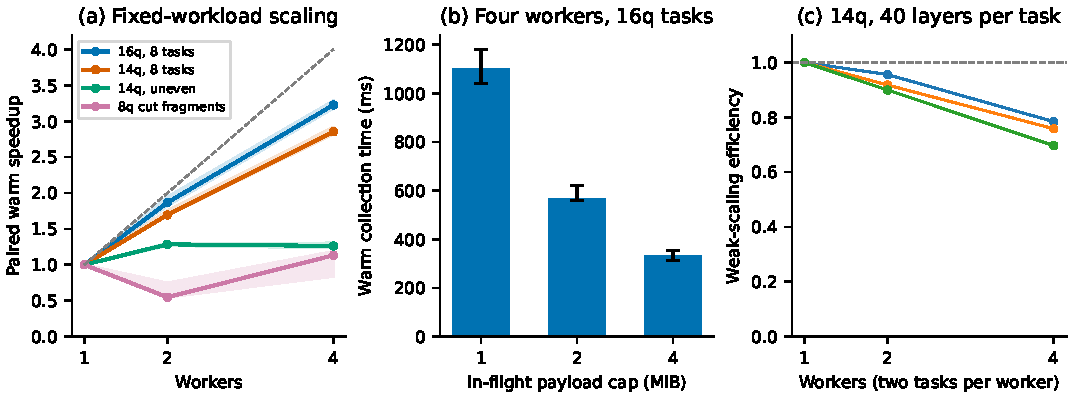
\includegraphics[width=\textwidth]{figures/local_parallel_scaling.pdf}
\caption{Measured local multiprocessing. (a) Fixed-workload speedups: lines show medians of three session-level paired geometric means; bands show their ranges, and the dashed line is ideal worker-count scaling. (b) Eight 16-qubit tasks on four workers under different aggregate payload caps: bars show medians of session medians, with session ranges. (c) Weak scaling holds two 14-qubit, 40-layer tasks per worker; each line is one session. All timings are warm and exclude setup.}
\label{fig:local_parallel_scaling}
\end{figure*}

\subsubsection{Strong Scaling and Task Granularity}
For each parallel policy, warm speedup is the geometric mean of paired serial/parallel time ratios; efficiency divides that speedup by the worker count. On eight 16-qubit components, four workers achieve $3.18\times$--$3.28\times$ speedup, corresponding to 79.6\%--82.1\% efficiency. Parallel median time is 313--355\,ms, while the separate one-worker configuration takes 1,028--1,169\,ms. The speedup uses paired serial controls within each pool configuration, so it need not equal the ratio of these independently summarized medians.

Eight balanced 14-qubit components reach $2.82\times$--$2.91\times$ on four workers. With only two components, four workers yield $1.68\times$--$1.71\times$: additional workers cannot create more independent tasks. An uneven eight-component batch, with seven four-layer components and one 80-layer component, yields only $1.24\times$--$1.30\times$. Its largest task limits completion time. Four-qubit components regress to $0.28\times$--$0.51\times$, while the connected bridge's cut fragments yield $0.84\times$--$1.19\times$. Thus the strongest scaling result concerns substantial independent tasks, not a demonstrated acceleration of connected-circuit cutting.

\subsubsection{Weak Scaling}
With two 14-qubit, 40-layer components per worker, the task count rises from two to eight as the worker count rises from one to four. Define weak-scaling efficiency as $T_1(2)/T_P(2P)$, using session median times. Four-worker efficiency is 69.7\%--78.4\%, and throughput grows from 29.7--32.4 to 90.0--93.5 tasks/s. The sublinear gain reflects the measured executor and shared host; it does not establish scaling beyond four processes.

\subsubsection{Setup Repayment and Time Allocation}
To assess short lifetimes, we sum the recorded first call and nine warm calls, adding construction, cold planning, and calibration once to both policies, plus full pool warmup and shutdown to parallel execution. This is cost accounting from interleaved observations, not a separately timed contiguous ten-call application. Full calibration takes 705--904\,ms per session; for the eight-task 16-qubit case, planning takes 210--343\,ms and four-worker warmup takes 103--146\,ms.

The 16-qubit workload retains a $2.56\times$--$2.63\times$ ten-call speedup with these charges, crossing break-even on the first recorded call in all three sessions. Eight balanced 14-qubit tasks retain $1.72\times$--$1.80\times$. In contrast, the shallow 14-qubit batch needs nine or ten calls to cross and ends at $1.00\times$--$1.02\times$; the ten-qubit batch remains slower despite its $1.19\times$--$1.25\times$ warm speedup. No later repayment is inferred for cases that do not cross within the observed horizon.

\begin{figure}[!t]
\centering
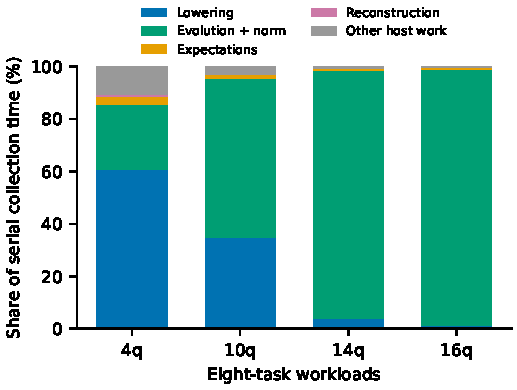
\includegraphics[width=\columnwidth]{figures/local_parallel_phases.pdf}
\caption{Time allocation in the one-worker configuration: mean per-call phase fractions over 27 warm observations per workload. Evolution includes initialization and norm checking. The residual includes host dispatch, cleanup, and instrumentation. These are serial wall-time fractions; parallel worker phase sums are not additive parent wall-time components.}
\label{fig:local_parallel_phases}
\end{figure}

Figure~\ref{fig:local_parallel_phases} explains the granularity dependence. Evolution and norm checking occupy approximately 25.0\% of serial collection time for the four-qubit workload, 60.9\% at ten qubits, 94.7\% at 14 qubits, and 98.0\% at 16 qubits. Native circuit lowering accounts for 60.8\% at four qubits. These workloads vary in depth as well as width, so the fractions characterize the tested configurations rather than a width-only law. Forced parallel execution avoids automatic-policy scoring, whose overhead remains visible: on the balanced eight-task 14-qubit workload, automatic dispatch achieves $2.58\times$--$2.62\times$, below forced parallelism.

\subsubsection{Memory, CPU, and Transport Costs}
For uniform independent tasks with payload $b$, worker count $P$, and aggregate payload budget $B$, at most $\min(P,\lfloor B/b\rfloor)$ tasks can be in flight, also bounded by available tasks. The 16-qubit states occupy 1\,MiB each. Holding four workers and the graph fixed, budgets of one, two, and four MiB yield speedups of $0.99\times$--$1.01\times$, $1.87\times$--$1.93\times$, and $3.18\times$--$3.28\times$, respectively (Fig.~\ref{fig:local_parallel_scaling}b). Provisioned processes alone do not supply usable parallelism when the payload budget serializes dispatch.

Resource measurements run in separate diagnostic collections to avoid sampling overhead in the timing trials. A 2\,ms target-period sampler reads Linux process RSS and CPU counters for the parent and the active pool. Summed sampled RSS counts shared pages once per process and may miss short peaks; it is neither unique physical memory nor an enforced RSS bound. CPU counters have 10\,ms resolution, so utilization ratios for probes shorter than 100\,ms are omitted.

For the eight-task 16-qubit workload, sampled parent-plus-pool RSS is 276--308\,MiB with four workers, compared with 147--174\,MiB serially, despite the much smaller four-MiB state-payload budget. Diagnostic CPU use is 1.29--1.38 CPU-s with four workers versus 1.04--1.14 CPU-s serially; lower latency does not imply less CPU work. The four-worker probes average approximately 3.85--4.01 CPU cores, including parent overhead. The four-worker pool still occupies roughly 276--308\,MiB when the payload cap is tightened, showing that payload throttling does not remove process overhead (Table~\ref{tab:local_parallel_resources}).

The eight 16-qubit task descriptions serialize to about 429\,KiB per collection before multiprocessing framing; results are scalar values and execution statistics. These are measured serialized object sizes, not monitored transport traffic. Numerical statevectors remain inside their executing process. The results therefore quantify a local multiprocessing trade-off among task granularity, available concurrency, setup repayment, and process footprint; they make no claim about networked or physical-QPU distribution.


% Generated by benchmarks/export_local_parallel_tables.py; do not hand-edit rows.
\subsection{Expanded Local Multiprocessing Artifacts}
The expanded study uses \path{benchmarks/run_local_parallel.py} with nine repetitions and
session indices zero through two. Raw data, plans, reference values, process samples, and source
fingerprints are in \path{results/local_parallel/session0/} through
\path{results/local_parallel/session2/}. The checked aggregate is
\path{results/local_parallel/summary.json}; its generator verifies source and graph
fingerprints. Workloads are fixed across sessions. Full calibration is charged to each workload
when calculating a standalone ten-call lifetime, although the measurement runner performs
calibration once per session. First-call and warm measurements are interleaved with controls;
unmeasured gaps are excluded from the summed cost model.

Table~\ref{tab:local_parallel_full} retains all ten workloads. $T_1$ and $T_4$ are ranges of
configuration-level median collection times. $S_2$ and $S_4$ are ranges of paired geometric-mean
speedups against serial controls measured within the corresponding pool configuration. $L_4$
includes common construction, planning, and calibration, plus parallel warmup, ten collections,
and shutdown. Bootstrap intervals for the nine paired trials in each session are retained in the
JSON, rather than conflated with session ranges. Three sessions on one host do not establish
between-machine uncertainty.

\begin{table*}[!t]
\caption{All Local Multiprocessing Workloads: Warm Timings, Paired Speedups, and Ten-Call
Setup-Charged Speedups. Ranges Span Three Sessions.}
\label{tab:local_parallel_full}
\centering
\footnotesize
\setlength{\tabcolsep}{4pt}
\begin{tabular}{lrrrrrrr}
\toprule
Workload & Tasks & $T_1$ (ms) & $T_4$ (ms) & $S_2$ & $S_4$ & $S_4/4$ & $L_4$ \\
\midrule
4q, 4 layers & 8 & 0.44--1.27 & 1.88--2.12 & 0.17--0.20 & 0.28--0.51 & 0.07--0.13 & 0.83--0.84 \\
10q, 20 layers & 8 & 9.95--11.27 & 8.93--10.76 & 0.83--0.88 & 1.19--1.25 & 0.30--0.31 & 0.89--0.91 \\
14q, 40 layers & 2 & 61.66--67.36 & 36.33--39.29 & 1.59--1.72 & 1.68--1.71 & 0.42--0.43 & 1.09--1.10 \\
14q, 40 layers & 4 & 114.50--130.81 & 39.18--42.63 & 1.63--1.74 & 2.76--2.91 & 0.69--0.73 & 1.38--1.50 \\
14q, 40 layers & 8 & 231.59--276.39 & 85.59--88.85 & 1.69--1.75 & 2.82--2.91 & 0.71--0.73 & 1.72--1.80 \\
16q, 40 layers & 8 & 1027.70--1168.86 & 312.80--355.16 & 1.82--1.94 & 3.18--3.28 & 0.80--0.82 & 2.56--2.63 \\
14q, 4 layers & 8 & 26.72--29.94 & 11.38--13.56 & 1.29--1.47 & 2.23--2.34 & 0.56--0.58 & 1.00--1.02 \\
14q, 80 layers & 8 & 452.12--474.31 & 159.90--162.88 & 1.71--1.74 & 2.73--3.03 & 0.68--0.76 & 1.84--2.08 \\
14q, uneven depths & 8 & 79.40--99.32 & 63.71--77.81 & 1.27--1.30 & 1.24--1.30 & 0.31--0.33 & 0.99--1.04 \\
8q cut fragments & 12 & 7.33--7.96 & 8.15--11.58 & 0.55--0.75 & 0.84--1.19 & 0.21--0.30 & 0.86--0.91 \\
\bottomrule
\end{tabular}
\par\vspace{8pt}
\caption{Resource Diagnostics for Eight 16-Qubit Tasks. Each State Occupies 1 MiB; Values Span
Three Separate Profiling Collections, One per Session.}
\label{tab:local_parallel_resources}
\centering
\footnotesize
\setlength{\tabcolsep}{5pt}
\begin{tabular}{rrrrrr}
\toprule
Workers & Payload cap (MiB) & Warm time (ms) & Sampled RSS sum (MiB) & CPU-s & Mean cores \\
\midrule
1 & 1 & 1027.70--1168.86 & 147.3--173.9 & 1.04--1.14 & 0.99--1.01 \\
2 & 2 & 562.61--654.97 & 213.4--239.0 & 1.19--1.61 & 2.03--2.10 \\
4 & 1 & 1039.75--1180.83 & 277.1--307.0 & 1.15--1.44 & 1.09--1.12 \\
4 & 2 & 558.94--622.99 & 276.3--307.6 & 1.14--1.67 & 2.07--2.13 \\
4 & 4 & 312.80--355.16 & 276.2--307.7 & 1.29--1.38 & 3.85--4.01 \\
\bottomrule
\end{tabular}
\end{table*}

The uneven case contains seven four-layer components and one 80-layer component. Other uncut
rows use the same depth per component. The cut row joins two eight-qubit, 20-layer components
with a CX bridge and adds terminal rotations. Scalar observables are validated using an
independent NumPy implementation; no sampled quantum execution is involved.

Warm timings in Table~\ref{tab:local_parallel_resources} come from unprofiled trials. RSS and
CPU columns come from separate instrumented collections. RSS is the sampled sum over the parent
and the active pool, including shared-page double counting and retained runtime allocations.
CPU-s sums user and system process counters; mean cores divides that CPU time by profiled
collection wall time and includes sampler/parent overhead. Raw process counters have 10 ms
resolution. All reported resource probes in this table exceed 100 ms; shorter workloads retain
raw counters but suppress derived utilization ratios. These measurements do not bound peak RSS
or measure energy.


\section{Artifacts and Provenance}
\label{app:provenance}
All raw observations, manifests and runners are part of the accompanying repository. The planner-versus-direct study is defined by \path{benchmarks/direct_baseline_manifest.json}. Its runners are \path{benchmarks/run_direct_baselines.py}, \path{benchmarks/run_gradient_baselines.py} and \path{benchmarks/run_memory_wall.py}, which share \path{benchmarks/direct_support.py}, and \path{benchmarks/summarize_direct.py} recomputes every reported median, ratio and figure from the raw rows in \path{results/direct/}. The GPU runners declare their dependencies inline, pinned by adjacent script lockfiles, and can be reproduced with \texttt{uv run --locked --script}. The same-backend comparison is \path{results/direct/backend_matrix.json}. The cloud confirmation ran \path{cloud/gpu-baselines.yaml} through \path{scripts/sky_gpu.sh} on a Lambda \texttt{gpu\_1x\_h100\_pcie} instance for 2\,h\,23\,min, and its results, including the host's \texttt{nvidia-smi} and \texttt{lscpu} records, are in \path{results/direct/remote/nvidia-h100-pcie/}. Each result file records the manifest hash, a hash of the package and runner sources, the command line, the thread settings, the CPU and GPU models and the package versions.

The QML matrix, the exhaustive grouping reference, the replay and parallel probes and the external backend pilots are in \path{results/qml_workloads/}, produced by the corresponding \path{benchmarks/run_qml_*.py}, \path{run_grouping_oracle.py}, \path{run_ionq_*.py} and \path{run_iqm_qml_*.py} runners and frozen in \path{benchmarks/qml_workload_manifest.json}. The interleaved comparison of the pre-study and current planners used in RQ3 is \path{results/qml_workloads/planner_ab/}, recomputed by \path{benchmarks/compare_planner_versions.py}; an earlier rerun in \path{results/qml_workloads/v2/} ran right after sustained GPU load, shows a uniform slowdown of its collections, and is not used. The analysis-budget coefficients are fitted by \path{benchmarks/calibrate_analysis_budget.py}, with its output in \path{results/analysis_budget/calibration.json}, and the Hamiltonian-averaging study of the budget is \path{results/analysis_budget/hamiltonian.json}, produced by \path{benchmarks/run_analysis_budget.py}. The earlier planning studies of Appendix~\ref{app:earlier} are in \path{results/p4_p5/}, \path{results/priorities/} and \path{results/workload_manifest/v2/}, with their analysis in \path{paper/analysis/}.

The generalization studies of Section~\ref{sec:generalization} are frozen in \path{benchmarks/qml_heldout_family_manifest.json}, \path{benchmarks/grouping_oracle_heldout_manifest.json}, \path{benchmarks/trained_iris_qml_v3_manifest.json} and \path{benchmarks/fourier_trained_qml_manifest.json}. The held-out screen runs as two sessions of \path{benchmarks/run_qml_depth_screen.py} and is summarized by \path{benchmarks/summarize_heldout_families.py}, which applies the analysis plan recorded in its manifest and checks the manifest hash of every session. The trained models come from \path{benchmarks/run_trained_iris_qml.py} and, for the replayed classifiers, \path{benchmarks/export_fourier_trained_models.py} followed by \path{benchmarks/run_fourier_trained_qml.py}. The exporter rebuilds every test split with the original study's code and refuses to continue unless its hash matches the one that study recorded. The tied-parameter control is \path{benchmarks/run_tied_qml_gradients.py}. The matched-basis IQM probes are \path{results/qml_workloads/iqm_garnet_basis_probe.json} and \path{results/qml_workloads/iqm_garnet_basis_probe_line.json}, produced by \path{benchmarks/run_iqm_qml_basis_probe.py} and summarized by \path{benchmarks/summarize_iqm_basis_probe.py}. \path{benchmarks/paper_generalization_tables.py} regenerates the corresponding tables from these results.

The revised beyond-device-memory study is defined by the \texttt{memory\_wall} section of \path{benchmarks/direct_baseline_manifest.json}. \path{benchmarks/run_memory_wall.py} now records exact global-MPS, reused-circuit tensor-network, LazyQC CPU and LazyQC GPU-placement timings, cone-width ranges, bond dimensions, validation errors, source hashes and environment fingerprints in \path{results/direct/memory_wall.json}. \path{benchmarks/summarize_direct.py} regenerates Tables~\ref{tab:memory-wall} and~\ref{tab:intermediate-cones} and their Markdown summaries from those rows. The direct Qiskit LightCone studies are frozen in \path{benchmarks/lightcone_ablation_manifest.json} and \path{benchmarks/lightcone_jacobian_manifest.json}, with runners \path{benchmarks/run_lightcone_ablation.py} and \path{benchmarks/run_lightcone_jacobian_ablation.py}. Their raw observations are \path{results/direct/lightcone_ablation.json} and \path{results/direct/lightcone_jacobian_ablation.json}; \path{benchmarks/summarize_lightcone_ablation.py} regenerates Table~\ref{tab:lightcone-ablation}. The policy comparison in Table~\ref{tab:policy-ablations} is a post-hoc analysis of the two frozen held-out session files, with no new timings: \path{benchmarks/summarize_policy_ablations.py} regenerates \path{results/qml_workloads/policy_ablations.json}, its Markdown report and the LaTeX table.

No immutable public release identifier is associated with these measurements yet.
